\documentclass[journal]{IEEEtran}
\usepackage{cite}
\usepackage[cmex10]{amsmath}
\usepackage{graphicx}
\usepackage{amssymb}
\usepackage{booktabs,multirow}
\usepackage{algpseudocode,algorithm2e}
% correct bad hyphenation here
\hyphenation{op-tical net-works semi-conduc-tor}


\begin{document}
%
% paper title
% can use linebreaks \\ within to get better formatting as desired
% Do not put math or special symbols in the title.
\title{Active Learning Based Constrained Clustering For Speaker Diarization}
%
%
% author names and IEEE memberships
% note positions of commas and nonbreaking spaces ( ~ ) LaTeX will not break
% a structure at a ~ so this keeps an author's name from being broken across
% two lines.
% use \thanks{} to gain access to the first footnote area
% a separate \thanks must be used for each paragraph as LaTeX2e's \thanks
% was not built to handle multiple paragraphs
%

\author{Chengzhu~Yu,~\IEEEmembership{Student~Member,~IEEE,}
        and John~H.~L.~Hansen,~\IEEEmembership{Fellow,~IEEE}}% <-this % stops a space
%\thanks{M. Shell is with the Department
%of Electrical and Computer Engineering, Georgia Institute of Technology, Atlanta,
%GA, 30332 USA e-mail: (see http://www.michaelshell.org/contact.html).}% <-this % stops a space
%\thanks{J. Doe and J. Doe are with Anonymous University.}% <-this % stops a space
%\thanks{Manuscript received April 19, 2005; revised December 27, 2012.}}

% note the % following the last \IEEEmembership and also \thanks - 
% these prevent an unwanted space from occurring between the last author name
% and the end of the author line. i.e., if you had this:
% 
% \author{....lastname \thanks{...} \thanks{...} }
%                     ^------------^------------^----Do not want these spaces!
%
% a space would be appended to the last name and could cause every name on that
% line to be shifted left slightly. This is one of those "LaTeX things". For
% instance, "\textbf{A} \textbf{B}" will typeset as "A B" not "AB". To get
% "AB" then you have to do: "\textbf{A}\textbf{B}"
% \thanks is no different in this regard, so shield the last } of each \thanks
% that ends a line with a % and do not let a space in before the next \thanks.
% Spaces after \IEEEmembership other than the last one are OK (and needed) as
% you are supposed to have spaces between the names. For what it is worth,
% this is a minor point as most people would not even notice if the said evil
% space somehow managed to creep in.



% The paper headers
\markboth{IEEE/ACM TRANSACTIONS ON AUDIO, SPEECH, AND LANGUAGE PROCESSING} %
{Shell \MakeLowercase{\textit{et al.}}: Bare Demo of IEEEtran.cls for Journals}
% The only time the second header will appear is for the odd numbered pages
% after the title page when using the twoside option.
% 
% *** Note that you probably will NOT want to include the author's ***
% *** name in the headers of peer review papers.                   ***
% You can use \ifCLASSOPTIONpeerreview for conditional compilation here if
% you desire.




% If you want to put a publisher's ID mark on the page you can do it like
% this:
%\IEEEpubid{0000--0000/00\$00.00~\copyright~2012 IEEE}
% Remember, if you use this you must call \IEEEpubidadjcol in the second
% column for its text to clear the IEEEpubid mark.



% use for special paper notices
%\IEEEspecialpapernotice{(Invited Paper)}


% make the title area
\maketitle

% As a general rule, do not put math, special symbols or citations
% in the abstract or keywords.
\begin{abstract}
Most speaker diarization researches focus on unsupervised scenarios, where no human supervision is available,. However, in many real-world applications, certain amount of human input could always be engaged, especially when minimal human supervision could brings significant performance improvement. Motivated by this, we propose an active learning based speaker clustering algorithm, to effectively improve speaker diarization performance with limited human input. Specifically, proposed algorithm has two different active learning components: \textit{explore} and \textit{consolidate}, acting in initial stages of bottom-up speaker clustering. While the concept of \textit{explore} and \textit{consolidate} are borrowed from the area of data mining, a substantial changes are made here for the application of speaker diarization. The main purpose of \textit{explore} and \textit{consolidate} stages in proposed algorithm, is to boost the speaker clustering process with reliably estimated initial speaker clusters. To achieve this, we uses farthest first query search (FFQS) with active learning to quickly discover at least one sample for each speaker during \textit{explore} phase, and employ nearest neighbor query search (NNQS) during \textit{consolidate} phase to ensure reliable instances for each discovered speaker cluster. After \textit{explore} and \textit{consolidate} phases, the standard bottom-up clustering is performed with a constraint that the clusters discovered during \textit{explore} phases are not merged with each other. Finally, we also propose an active learning based cluster reassignment approach, where clustered segments that accounted for largest expected speaker error are chosen for human evaluation. We evaluate the proposed algorithm on a subset of Apollo multi-track corpus and AMI meeting corpus. The results indicate significant improvement of speaker diarization performance with relatively small amount of human supervision.  
     
\end{abstract}

% Note that keywords are not normally used for peerreview papers.
\begin{IEEEkeywords}
Speaker diarization, active learning, bottom-up clustering
\end{IEEEkeywords}

% For peer review papers, you can put extra information on the cover
% page as needed:
% \ifCLASSOPTIONpeerreview
% \begin{center} \bfseries EDICS Category: 3-BBND \end{center}
% \fi
%
% For peerreview papers, this IEEEtran command inserts a page break and
% creates the second title. It will be ignored for other modes.
\IEEEpeerreviewmaketitle

\section{Introduction}
Speaker diarization is the process of automatically detecting \textit{who spoke when }in an audio sequence. With increasing amount of audio resources, speaker diarization becomes an important technology in many applications such as information retrieval, metadata extractions, meeting annotations, and conversation analysis. Recent developments for speaker diarization algorithms have been largely driven by Rich Transcription (RT), where speaker diarization plays a role to provide speaker index and other information to achieve improved speech-to-text transcriptions.

As a sequential process, speaker diarization normally involves several components such as voice activity detection, speaker change detection (segmentation), clustering, and re-segmentation. Among theses components, the core of speaker diarization is clustering, where it separate segments from different audio sources such as speaker, music, and noise, and group them together. Due to its significance in speaker diarization, various solutions have been proposed for speaker clustering. Theses include but not limited to bottom-up approach, also known as agglomerative hierarchical clustering (AHC), top-down approach, and recently proposed global optimization approaches. 

Bottom-up clustering is in general the most popular strategy among various clustering solutions. It starts by treating each individual segments, obtained in the segmentation stage, as separate clusters, and iteratively merging the closest two clusters until a specified stopping criteria is satisfied. While not as popular as its counterpart, top-down approach has also been applied widely and some studies have reported that it could achieve comparable result as bottom-up clustering [Evans, 2012]. Different from bottom-up based approach, top-down clustering starts from modeling the entire audio as single model and iteratively splitting the model into sub clusters until a stopping criteria is met. Despite their differences, both bottom-up and top-down based approach are iterative process and has the drawback of error propagation. A recently proposed clustering algorithm, Interger Linear Programming (ILP), attempts to overcome this drawback by finding the cluster assignments that jointly minimizing the number of assigned clusters as well as within-cluster dispersion. While the ILP could avoid the drawbacks of error propagation, it has to start with initial clusters that contains sufficient samples for estimating its characteristic (e.g., i-vector). Therefore, ILP is mostly performed on top of a bottom-up clustering.

Along with the development in speaker clustering, the distances metric for performing speaker clustering has also made significant improvement from original Bayesian informative criteria (BIC), generalized log-likelihood ration (GLR), Kullback-Leibler (KL) divergence, to recent i-vector based distances such as cosine distance score (CDS) as well as probablistic linear discriminant analysis (PLDA) based distance. Other alternative distance metrics, such as these based on information theoretic framework are also proposed and showed competitive results. 

Despite the success of recent improvement on speaker clustering algorithms, distance computations, as well as other non-trivial components, speaker diarization still remained as challenging tasks in many real-word applications, especially where the audio quality is suboptimal or the speech communications comprises large proportions of fast speaker turns. For example, diarization of telephone conversations are notably more challenging compared with broadcast news diarization, as well as meeting room diarization. 

Due to the limitation within current speaker diarization systems using exclusively audio/speech information, a number of recent studies have proposed to exploit auxilary informations for improved speaker diarization performance. For example, the linguist information such as speaker name occurring patterns are extracted from the speech transcripts to provide additional information during speaker clustering. The speech transcript could be obtained from manual transcript as well as automatic speech recognition system. Another important supplementary information that presents in many speaker diarization applications is the visual information. The audio-visual speaker diarization has also been studied.

In this study, we propose an active learning based, bottom-up speaker clustering algorithm that effectively utilize human input to improve speaker diarization performance. Our proposed algorithm is based on an assumption that human input could be engaged during speaker diarization process in certain applications. This scenario is especially plausible if small amount of human engagement could brings significant performance improvements. Another assumption we made in this paper is that, human is better than machine for recognizing whether a given segment pair is from the same speaker or not. This assumption is based on the results from previous studies that while current speaker recognition systems shows competitive performance as human in clean speech condition, in adverse conditions human significantly outperform machine. Besides, many audio streams for speaker diarization applications contain higher level information such as video, spoken names, and contextual informations that could effectively employed by human for determining whether the two segments are from the same speaker or not.

The format of query for human to provide ground truth in speaker diarization, is \textit{yes or no} type of question asking whether a given segments pair belongs to the same speaker or not. The total number of queries for obtaining perfect clustering results requires $O(N^{2})$, where N indicates the number of segments. Therefore, an effective active query selection strategy is necessary in order to effectively employ human input to boosting the speaker diarization performance. 

To effectively employ human input, we first need to identify which part of speaker clustering components has most effect on final speaker diarization performance. In other words, involving human input in which part of current speaker clustering algorithm, could most effectively improve the overall speaker diarization performance. A recent study by [Simon King] has evaluated several key components of speaker diarization and concluded that initialize speaker models with pure and reliably labeled data could lead to significant improvement to the overall speaker diarization performance.   Motivated by the above findings, we designed our active learning algorithm to quickly discover all or most of the speakers in audio stream in the \textit{explore} phase, and ensure sufficient and reliable samples for each cluster to during \textit{consolidate} phase. The initial speaker models for trained after explore and consolidate phases are much reliable than those obtained in fully unsupervised manner, and are expected to lift the speaker clustering process.

In addition to active learning for improved speaker clustering process, we also investigate the use of active learning for cluster reassignment approach. The objective of proposed cluster reassignment approach, is to actively select certain speech segments from clustered result for human evaluation/correction. The key of active learning based cluster reassignment, is to effectively find most informative segments, from current clustering results. In this study, we find speech segments with largest expected speaker error difference as a candidates for human evaluation.

To summary, in this study, we investigate the use of active learning for bottom-up clustering stage of speaker diarization. We proposed two different strategies where active learning are employed for robust initial cluster estimation and post clustering reassignment, respectively. The remainder of paper is organized as follows.   

\begin{figure*}
	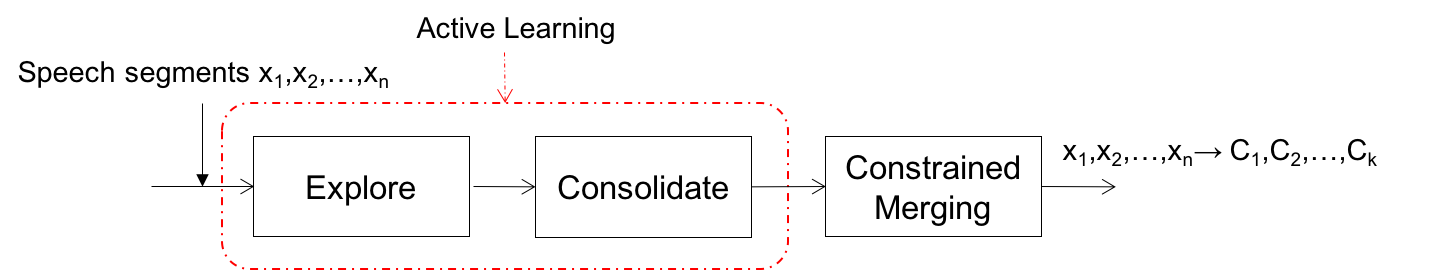
\includegraphics[width=\linewidth]{figs/flow3}
	\caption{A boat.}
	\label{fig:boat1}
\end{figure*}

\section{Related Work}
Active learning based constrained clustering has been extensively studied for image clustering tasks and in broader area of data mining. A number of active learning algorithms have been proposed to use active learning for clustering unlabeled data with human in the loop. The key idea behind these algorithms is to actively select pairs of data for human to provide answer in a form of yes or no. 
Most of the algorithms proposed in these studies, are targeting k-means clustering, and normally composed of two stage: \textit{explore} and \textit{consolidate}. The purpose \textit{explore} phase is to find the centroids of different clusters, and the aim of consolidate stage is to locate most informative data pair for human labeling. While the fundamental problem of these studies is much similar to the problem we have in speaker diarization, active learning for speaker diarization is more challenging task in general due to the two reasons. Firstly, the bottom-up clustering in speaker diarization requires to iteratively clustering two closest segments and update the cluster statistics after each iteration. Therefore, the decisions in current iteration has reliance on previous iteration, and therefor it is difficult to quantify the importance of each segment pair. Another important difference is that, the total number of cluster numbers in speaker diarization are unknown most of time. Due to these differences, the direct replication of active learning algorithms developed in these studies, is not viable.

On the other hand, only a limited number of studies in the area of speaker recognition and diarization, has investigates the use of active learning for speaker diarization tasks. For example, the study by [Shum] has investigate to use active learning to obtain background speaker labels from unlabeled data for training PLDA system. While the study by [Shum] bears similarity with this paper, but the ultimate goal of [Shum] is to locate reliable samples sufficient enough to train PLDA system, rather than clustering entire data as in speaker diairization task. Another study, that employ active learning for speaker diarization is by [Mateusz], where the criteria of active selection for human labeling is simply based on the length of speech, which will not work in many speaker diarization task where the variance of segment length is small.

\section{Baseline System}
The baseline speaker diarization used in this study, is a bottom-up speech clustering algorithm with i-vector cosine distances score as distance metric between two speech segments. In this section, we will give a brief discussion about i-vector extraction, cosine distance score (CDS) and bottom-up clustering approach. 

\subsection{i-vector extraction}
In i-vector extraction framework, speaker and channel dependent GMM supervector is modeled as follows:
\begin{equation}
\begin{aligned}
& M=m+Tw,
\label{mmtw}
\end{aligned}
\end{equation}
where $m$ is the supervector obtained from the universal background model (UBM), 
$T$ is the low rank total variability matrix representing the basis of reduced total variability space, 
and $w$ is the low rank factor loadings referred to as i-Vectors. 

The estimation of the total variability matrix $T$ employs expectation maximization (EM) method as described in \cite{kenny2005eigenvoice}. 
After training the total variability matrix, 
the i-Vector of given speech utterance is extracted as the conditional expectation of i-Vector distribution given observation features.
\begin{equation}
\begin{aligned}
&w_{s}^{\ast}=E[P(w_{s}|X_{s})],
\label{eq:ws}
\end{aligned}
\end{equation}
where $w_{s}^{\ast}$ is the i-Vector of the given speech utterance $s$, 
$X_{s}$ is the clean observation features, 
$P(w_{s}|X_{s})$ is the conditional distribution of the i-Vector given observation features, 
and $E[\cdot]$ indicates the expectation. 
Finally, the i-Vector of the given speech utterance can be represented using the Baum-Welch zeroth ($N_s$) and centralized first ($F_s$) order statistics,
\begin{equation}
\begin{aligned}
&w_{s}^{\ast}=(T'N_{s}\Sigma^{-1}T+I)^{-1}T\Sigma^{-1}F_{s},
\label{ws2}
\end{aligned}
\end{equation}
where $\Sigma$ is the covariance matrix obtained from UBM model and $I$ is the identity matrix.

\subsection{Cosine Distance Score}
Comparison  i-vectors from two different segments, could be successfully achieved with simple cosine similarity. The cosine distance score between two vectors could be expressed as follow:
\begin{equation}
\begin{aligned}
& score (w_i, w_j) = \dfrac{w^T_i \cdot w_j}{\rvert\rvert{w_i}\rvert\rvert \cdot \rvert\rvert{w_j}\rvert\rvert}.
\label{ws2}
\end{aligned}
\end{equation}
Note that, the score of cosine distance ranges between [-1, 1]. The higher the number towards 1, the more similarity exist between two vectors. The cosine distance score has been a popular metric for speaker recognition and verification in i-vector space.
 
\subsection{Bottom-up Speaker Clustering}
Bottom-up clustering, also known as hierarchical agglomerative clustering, has been the most popular speaker clustering algorithm used for speaker diarization. It typically start by treating all homogeneous segments as a separate cluster, and iteratively merge two closest clusters. In our study, for each iteration, we find two segments that has the highest cosine similarity, and merge them into a single cluster. After each iteration, i-vectors of all segments are normalized to have zero mean. We continue the iteration until CDS of two closest segment reached stopping criteria. 

\section{Active Learning for Cluster Initialization}
Due to the error propagation characteristics of bottom-up speaker clustering, having good initial cluster model, with pure speaker segments in each clustering, has significant impact on the final speaker diarization performance. In this section, we will give a detailed description of our proposed active learning strategy for cluster initialization. As mentioned in Introduction, the proposed algorithm has two active learning components: \textit{explore} and \textit{consolidate}.

\begin{figure*}
	
\includegraphics[width=\linewidth]{figs/flow4}
	\caption{A boat.}
	\label{fig:boat1}
\end{figure*}

\subsection{Explore}
The purpose of explore phase, is to quickly discover all the speaker clusters within the audio streams, finding at least one speech segment for each speaker cluster. To achieve this, we use the farthest first query search (FFQS) proposed by [Basu]. Specifically, a speech segment is randomly selected from all speech segments to be used as seed segment. The selected speech segment is then used to initialize the first cluster. After creating the first speaker cluster, the next segment is selected which is farthest from existing clusters. The chosen segment is then provided for human to provide expert opinion. If the chosen segment belongs to existing clusters after pairwise comparison, the new segment is merged to the corresponding cluster. Otherwise, a new cluster is created from the selected segment. Note that, in order to decided if a given speech segment belongs to a target cluster or not, we compose a query pair using the segment in question and the longest segment within the target cluster. If the answer returns by human expert is true, then the segment belongs to the target cluster, and vice versa. The FFQS process continues until the pairwise comparison operations reached specified maximum number specified by user.   
 
\begin{algorithm}
	\KwData{Set of speech segments $X = {\{x_i\}}_{i=1}^n$, acess to the answers of pairwise queries, maximum number queries $Q$ user specified. }
	\KwResult{$C_{k=1}^{k}$ initialized clusters}
	Start from null cluster $C= \{\}$\;
	Select a segment $x$ at random, and create the first cluster as $C_1 = \{x_i\}$, $\lambda \leftarrow 1$\; 
	\While{maximum queries not reached, $\lambda < Q$}{
		Find speech segment $x_{\lambda}$ farthest from existing clusters in $C$, based on i-vector cosine similarity scores.\;
		\eIf{$x_{\lambda}$ belongs to any clusters in $C$}{
			Add speech segment $x_{\lambda}$ to cluster matching cluster
		}{
			Create new cluster $C_k$ with speech segment $x_{\lambda}$\;
		}
		Increase $\lambda$, for each query access. 	
	}
	\caption{FFQS with random seed during \textit{explore} phase.}
\end{algorithm}
 
While the above algorithms could effectively explore the speaker clusters in the audio streams, its performance varies a lot depending on which seed segment is selected. This problem is due to the randomness during seed selection. The previous studies in k-means clustering has revealed that, the initial seed data should be closer to actual centroids in order to achieve favorable clustering results. Motivated by this, we first performed a fully unsupervised bottom-up clustering on the entire speech segments, and taking the centroid segment of each cluster as initial active selection candidates to start FFQS algorithm during \textit{explore} phase.

\subsection{Consolidate}
The FFQS during \textit{explore} stage is very effective in discovering all involved speaker with given audio stream. However, it is not effective, when we need to quickly gather enough instances for each cluster to obtain reliable speaker models. For this purpose, for each discovered clusters obtained from \textit{explore} stage, we uses a nearest neighbor query search (NNQS) approach, to select speech segments closest to it for human evaluation.  

\begin{algorithm}
	\KwData{$C_{k=1}^{k}$ initialized clusters, set of speech segments $X = {\{x_i\}}_{i=1}^n$, acess to the answers of pairwise queries, maximum number queries per cluster $Q_k$ user specified. }
	\KwResult{$C_{k=1}^{k}$ with more instances.}
	\For{each cluster $C_k$ in $C_{k=1}^{k}$}{
		\While{maximum queries per cluster $Q_k$ not reached}{
			Find speech segment $\textbf{x}$ closest from $C_k$, based on i-vector cosine similarity scores.\;
			\eIf{$\textbf{x}$ belongs to any clusters in $C_k$}{
				Add speech segment $\textbf{x}$ to cluster $C_k$
			}{
				Exlude this segment $\textbf{x}$ from search in next iteration.
			}
		}
	}
	\caption{NNQS algorithm during \textit{consolidate} phase.}
\end{algorithm}

\subsection{Constrained Merging}
After \textit{explore} and \textit{consolidate} phases, the standard bottom-up clustering is performed with two important exceptions. First, the clusters $C_{k=1}^{k}$ created during \textit{explore} and \textit{consolidate} stages, are restricted to not merge with each other. Second, the stopping distance threshold during bottom-up clustering is no longer necessary, as we have assumed all involved speakers are discovered during \textit{explore} phase. The bottom-up clustering will continues until only $C_{k=1}^{k}$ clusters remain.

\section{Active Learning for Cluster Reassignment}
In previous section, we propose an active learning based algorithm to obtain better initial speaker models. Alternatively, human input could be involved after clustering finishes, to evaluate and fix incorrectly assigned clusters. This is quite similar to the use of active learning for automatic speech recognition (ASR), where the sentence with less confidence is passed to human for correction. However, the same algorithm used for ASR could not be directly applied in speaker diarization for several reasons. First, the confidence measure used for ASR is not appropriate for speaker diarization. Second, assuming we have identified potential erroneous segments, the human evaluation for evaluate and reassign these segments are much more complex than human transcription in ASR.

The proposed active learning based cluster reassignment has three major components that we will explain in this section. 

\subsection{Candidates selection}
The cluster reassignment algorithm starts with selecting the candidate speech segments and its assigned cluster for human expert to review later. In order to effectively select most informative segments, we ranks all speech segments in terms of expected speaker error reduction. In other words, we will select the speech segments that will produce largest expected speaker error reduction. 
The expected speaker error for each speech segment could be computed as below. 
\begin{equation}
\begin{aligned}
E(x_j) =& P(x_j | C_j) \cdot J_{x_j \in C_j} \\
&+ (1 - P(x_j | C_j)) \cdot J_{x_j \notin C_j}
\label{expect}
\end{aligned}
\end{equation}

where $x_j$ indicates $j$th speech segment, $C_j$ is the cluster assigned to speech segment $x_j$, $P(x_j|C_j)$ is the probability of segment $x_j$ belongs to cluster $c_j$, $J_{x_j \in C_j} $ is the speaker error if $x_j$ belongs to cluster $C_j$, and $J_{x_j \notin C_j}$ is the speaker error if $x_j$ not belongs to cluster $C_j$. We could also write that
\begin{equation}
\begin{aligned}
&J_{x_j \in C_j} = 0 \\
&J_{x_j \notin C_j} = \dfrac{d_j}{\sum_{i=1}^{n} d_i}
\label{jj}
\end{aligned}
\end{equation} 
where $d_j$ is the length of speech segment $x_j$, and $\sum_{i=1}^{n} d_i$ is total length sum of all speech segments of the testing audio stream.

We compute $P(x_j|C_j)$ by modeling a multivariate Gaussian distribution for each $C_{k=1}^{k}$ using i-vectors of all the segments of given cluster. We normalize the probability to sum to one.
\begin{equation}
\begin{aligned}
&  \sum_{i=1}^{k} P(x_j|C_i) = 1;
\label{jj}
\end{aligned}
\end{equation}
 
\begin{figure}[t]
	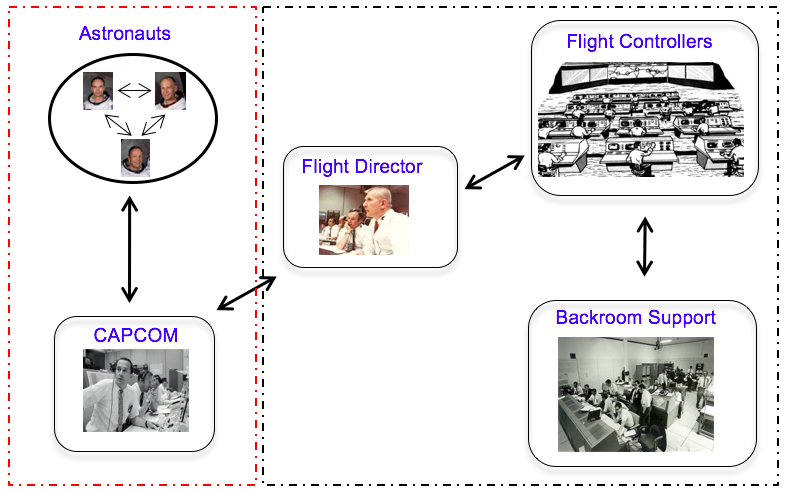
\includegraphics[width=\linewidth]{figs/comm5}
	\caption{A boat.}
	\label{fig:boat1}
\end{figure}

\subsection{Evaluation}
After selecting the candidate segments, human expert will determine whether the given segment belongs to its assigned cluster. The process of employing human input to decide whether a segment belongs to a cluster, is more difficult than the strategy we used in \textit{explore} and \textit{consolidate} phases of previous section. We could not compose query pair with the segment in question and a single longest segment in the cluster. This is due to the fact that the chosen longest segment of the cluster, could also be an incorrect assignment. Therefore, we employ a majority voting based segment cluster evaluation strategy. Under this strategy, the segment in question is paired with each segments within assigned cluster, resulting in multiple query pairs. If majority answers of these pairs are true (two segments belong to the same cluster), we will make a decision that the given speech segment has correct cluster assignment, and vice versa. 

While the above strategy is robust for evaluating whether a given segment belongs to target cluster, it involves significant number of query pair for human evaluation. One heuristic that we used in our study to effectively reduce the query pair number is to set a maximum query number limit $V$ for each segment evaluation. We rank each segments with the target cluster by its confidence $P(x|c)$, and select top $V$ confident segments for composing pairs with test segment. 

\subsection{Correction}
After detecting segments with incorrect cluster assignment in \textit{evaluation} stage, we need find the correct cluster designation for these segments. To achieve, we employ N-best cluster evaluation.
We find the $N$ most possible cluster candidates for given segment by ranking the i-vector Gaussian posterior probabilities $P(x|C)$. The human expert will evaluate in order whether the given segment belongs to any of these N clusters, using the majority voting scheme as in the \textit{evaluation} stage. 

\section{Test Data}
We performs experiments on two different speech database: Apollo-11 Mission Control Center (MCC) audio  corpus and AMI meeting corpus. 

\begin{figure}[t]
	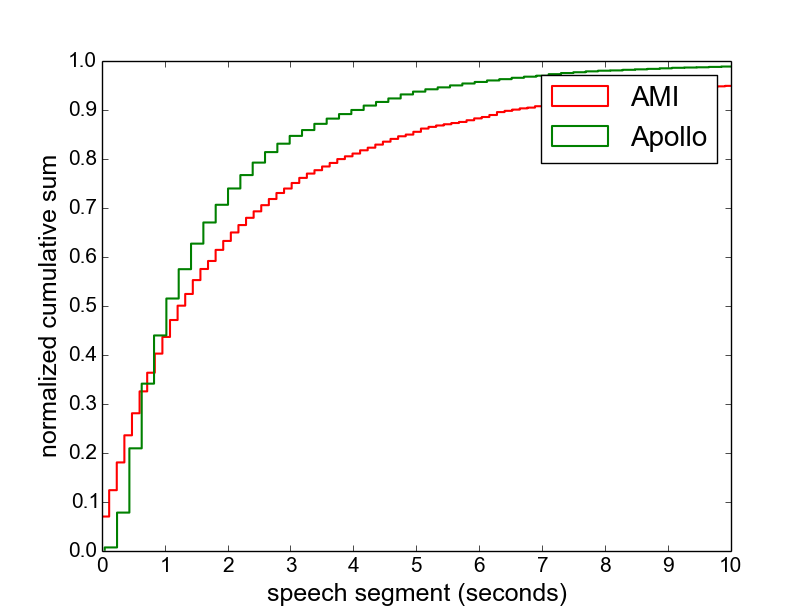
\includegraphics[width=\linewidth]{figs/lens}
	\caption{A boat.}
	\label{fig:boat1}
\end{figure}


\subsection{Apollo-11 MCC Audio Corpus}
During the NASA Apollo mission, all communications between astronauts, flight controllers inside mission control center (MCC), and their backroom support teams are continuously recorded using a 30-track analog reel-to-reel recording machine. During each mission, a total of 60 audio channels are simultaneously recorded including the voices from more than hundred of different participants of the mission. The University of Texas at Dallas (UTD), University of Maryland College Park (UMD), and Johnson Space Center(JSC) has combined the effort to digitize this data resource and have generated up to 19,000 hours of audio data from various missions of both Apollo and Gemini missions. Those mission audio records the full detail of the Apollo communication, therefore extremely attractive for learning human-to-human communications, group interaction, as well as developing robust speech system. 

Moreover, as the speech community (including us) rely on labeled audio data to perform scientific research as well as algorithmic development, we have prepared a 'Task Specific' corpus based on a subset of Apollo-11 audio recordings. We performed our experiment on this subset of Apollo-11 audio recordings includes 3 synchronized channels
(Flight director loop, EECOM loop, GNC) spanning 10-hours before, and after lunar landing. This initial 30 hour task corpus has been transcribed to have speaker labels by well-trained speech science students from UTDallas \footnote{The task corpus will be released to the speech community for research and algorithmic development.}.

The audios in Apollo-11 MCC audio corpus includes two types of communication: space-to-ground communications between astronauts and CAPCOM, and ground communication between flight directors and "backroom" support staff. Most of the audios are recorded with close-talking microphones and the audios are in general good quality. The audios from astronauts transmitted through Earth's dedicated telephone channels to Houston from ground stations where the signal was received. The flight directors as well as their "backroom" supports' voice are recorded through intercom circuit called "loops". Each flight director has their own loops, which records the entire communication within that channel.

The voice communication style withing Apollo mission control center is much different from both traditional meeting corpus, including many short speech segments which was intended to improve communication efficiency. 

\begin{table}[t]
\centering
\caption{My caption}
\label{my-label}
\small
\begin{tabular}{|c|c|c|c|}
\hline
Session Name & Speech (seconds) & Speech Segments & Participants \\ \hline
FD-01        & 252              & 161             & 9            \\ \hline
FD-02        & 314              & 152             & 9            \\ \hline
FD-03        & 123              & 63              & 10           \\ \hline
FD-04        & 651              & 358             & 13           \\ \hline
FD-05        & 457              & 226             & 14           \\ \hline
FD-06        & 979              & 531             & 12           \\ \hline
FD-07        & 394              & 267             & 13           \\ \hline
FD-08        & 486              & 340             & 15           \\ \hline
FD-09        & 217              & 126             & 13           \\ \hline
FD-10        & 964              & 713             & 13           \\ \hline
EECOM-01     & 1206             & 585             & 20           \\ \hline
EECOM-02     & 563              & 252             & 20           \\ \hline
EECOM-03     & 1014             & 471             & 31           \\ \hline
EECOM-04     & 808              & 384             & 20           \\ \hline
EECOM-05     & 812              & 357             & 26           \\ \hline
EECOM-06     & 475              & 270             & 23           \\ \hline
EECOM-07     & 553              & 337             & 21           \\ \hline
EECOM-08     & 411              & 261             & 19           \\ \hline
EECOM-09     & 744              & 430             & 31           \\ \hline
GNC-01       & 859              & 270             & 17           \\ \hline
GNC-02       & 735              & 346             & 21           \\ \hline
GNC-03       & 653              & 291             & 25           \\ \hline
GNC-04       & 1347             & 494             & 20           \\ \hline
GNC-05       & 798              & 440             & 21           \\ \hline
GNC-06       & 985              & 456             & 24           \\ \hline
GNC-07       & 829              & 481             & 24           \\ \hline
GNC-08       & 764              & 435             & 29           \\ \hline
GNC-09       & 1728             & 995             & 29           \\ \hline
\end{tabular}
\end{table}

\subsection{AMI Meeting Dataset}
We also evaluate proposed algorithms in the popular 12-meeting subset of Augmented MultiParty Interaction (AMI) corpus. This is approximately 5.4 hours of data with each session varying between 15-30 minutes. The AMI corpus contains both audio and visual data, and we uses only the audio data recorded with headset microphones in our experiments. The corpus represents a natural meeting scenarios. A total of four participants are involved in each session, discussing about the task to design a new new remote control device.  

\section{Experiments and Results}
In this section, we will perform experiments to evaluate proposed active learning based algorithms for speaker diarization. 
\subsection{System Setup}
\subsection{Active Learning Based Cluster Initialization}
\subsection{Active Learning Based Cluster Reassignment}

\section*{Acknowledgments}
This research was supported by National Science Foundation (NSF) under Grant 1219130.
 


\appendices
\section{Proof of the First Zonklar Equation}
Appendix one text goes here.

% you can choose not to have a title for an appendix
% if you want by leaving the argument blank
\section{}
Appendix two text goes here.


% use section* for acknowledgement
\section*{Acknowledgment}


The authors would like to thank...


% Can use something like this to put references on a page
% by themselves when using endfloat and the captionsoff option.
\ifCLASSOPTIONcaptionsoff
  \newpage
\fi

\bibliographystyle{IEEEtran}
\bibliography{IEEEabrv,MOREabrv,strings,ref}


\end{document}


